% 原书 p.323–p.330（PDF p.331–p.338）

% >>> p331
为结束本节，让我们提出以下几个问题，它们将在下一节中得到完整回答。

\begin{wque}{10.6.2}
  哈密顿微分同胚的作用（比如作用在拉格朗日子流形上）如何转化为其层对应物上的运算？
  反过来，层上的层运算是否启发拉格朗日子流形上的某些运算？
\end{wque}

\section{奇性支撑（II）（Singular Support (II)）}

\begin{keytakeaways}
\begin{itemize}
  \item 几何图像：奇性支撑 $SS(\mathcal F)$ 可以完全由「传播」的失败来刻画——在
        点 $(x,p)$ 处，若沿某个检验函数 $\varphi$（$\varphi(x)=0$、$\mathrm d\varphi(x)=p$）
        的「正侧」做上同调总为零，则层在该点传播；不传播的点构成 $SS(\mathcal F)$。
  \item 数学工具：新函子 $\Gamma_Z$ 与半正合列 (10.39)、命题 10.7.1 的传播判据、
        定义 10.7.1 的导出版本；以及 $SS$ 在 $f^{-1}$、$Rf_*$、$Rf_!$、$\otimes$、
        $R\mathcal H om$ 下的函子性（命题 10.7.2、10.7.3）。
  \item 关键构造：层卷积 $*$（式 (10.46)）与层复合 $\circ$（式 (10.48)）；层复合
        在几何上对应拉格朗日对应 (10.49)，即
        $SS(\mathcal F\circ\mathcal G)\subset SS(\mathcal F)\circ SS(\mathcal G)$
        （式 (10.50)）。
  \item 与辛几何的联系：$SS$ 把层的六种运算翻译为 $T^*X$ 中的集合运算，这正是
        10.8 节用 GKS 层量子化证明 Arnold--Givental 猜想的语言基础。
\end{itemize}
\end{keytakeaways}

本节开始，我们先补上定理 10.6.1 中的缺口：对
$\mathcal F=\mathcal F^\bullet\in\Op{Ob}(D(\Op{Sh}(\mathbf{k}_X)))$，如何定义
$SS(\mathcal F)$？为此引入一个新函子
\begin{equation}\tag{10.38}
  \Gamma_Z\colon\Op{Sh}(\mathbf{k}_X)\to\Op{Sh}(\mathbf{k}_X),
\end{equation}
定义如下：若 $Z\subset X$ 是开的，则 $(\Gamma_Z\mathcal F)(U)
:=\mathcal F(U\cup Z)$；若 $Z\subset X$ 是闭的，则
$(\Gamma_Z\mathcal F)(U):=\ker\bigl(\mathcal F(U)\to\mathcal F(U\setminus Z)\bigr)$
（其中 $U\setminus Z$ 是开的）。因此，若 $Z$ 是闭的，按定义有半正合列
\begin{equation}\tag{10.39}
  0\to\Gamma_Z\mathcal F\to\mathcal F\to\Gamma_{X\setminus Z}\mathcal F.
\end{equation}
一般地，函子 $\Gamma_Z$ 只是左正合的。利用这一记号，可以把定义 10.6.1 中的传播
条件重新表述如下。

\begin{wprop}{10.7.1}
  层 $\mathcal F\in\Op{Ob}(\Op{Sh}(\mathbf{k}_X))$ 在 $(x,p)\in T^*X$ 处传播，
  当且仅当对任何满足 $\varphi(x)=0$、$\mathrm d\varphi(x)=p$ 的函数
  $\varphi\colon X\to\R$，都有 $H^*\bigl(\Gamma_{\{\varphi(x)\ge0\}}\mathcal F
  \bigr)_x=0$。
\end{wprop}

% [Tutor Note: 易错预警——$\Gamma_Z$ 的正合性依赖 $Z$ 的拓扑类型：当 $Z$ 开时，
% $\Gamma_Z$ 只是「限制到 $U\cup Z$」，它是正合函子；当 $Z$ 闭时，
% $\Gamma_Z$ 是「支撑在 $Z$ 中的截面」，它只左正合，其高阶导出函子
% $R^i\Gamma_Z$ 一般不为零——这正是 (10.39) 只是「半正合列」且证明中需要
% 导出函子 $R^i\Gamma(U,\cdot)$ 的原因。另注意 (10.39) 的第三个对象是
% $\Gamma_{X\setminus Z}$（$X\setminus Z$ 是开集），而不是 $\Gamma_Z$ 的商。]

\begin{wrem}{10.7.1}
  我们需要对记号 $H^*\bigl(\Gamma_{\{\varphi(x)\ge0\}}\mathcal F\bigr)_x$ 作
  些解释。对任何 $U\in\operatorname{Op}(X,x)$，考虑对应
  \[
    H^*\bigl(U;\Gamma_{\{\varphi(x)\ge0\}}\mathcal F\bigr)
    :=H^*\circ R\Gamma(U,\cdot)\circ\Gamma_{\{\varphi(x)\ge0\}}\mathcal F,
  \]
  它给出一个（$\mathbf{k}$-模的）预层。于是按茎的定义，
  \[
    H^*\bigl(\Gamma_{\{\varphi(x)\ge0\}}\mathcal F\bigr)_x
    =\lim_{U\in\operatorname{Op}(X,x)}H^*\bigl(U;
    \Gamma_{\{\varphi(x)\ge0\}}\mathcal F\bigr).
  \]
  用同样的方式可以定义
  $H^*\bigl(\Gamma_{\{\varphi(x)<0\}}\mathcal F\bigr)_x$ 与
  $H^*(\mathcal F)_x$。
\end{wrem}

命题 10.7.1 的证明有点复杂，这里我们只给出证明梗概，并省略一些步骤。

\begin{wproof}[命题 10.7.1 的证明]
  假设我们有如下短正合列
  \begin{equation}\tag{10.40}
    0\to\Gamma_{\{\varphi(x)\ge0\}}\mathcal F\to\mathcal F
    \to\Gamma_{\{\varphi(x)<0\}}\mathcal F\to0,
  \end{equation}

% >>> p332
  而实际上最后一个箭头
  $\Gamma_{\{\varphi(x)<0\}}\mathcal F\to0$（满射性）可能不成立。作用第 $i$ 个
  导出函子 $R^i\Gamma(U,\cdot)$，得到长正合列：
  \[
    0\to\bigl(\Gamma_{\{\varphi(x)\ge0\}}\mathcal F\bigr)(U)
    \to\mathcal F(U)\to\bigl(\Gamma_{\{\varphi(x)<0\}}\mathcal F\bigr)(U)
    \to R^1\Gamma\bigl(U;\Gamma_{\{\varphi(x)\ge0\}}\mathcal F\bigr)\to\cdots,
  \]
  它等价于 $\mathbf{k}$-模的长正合列
  \[
    \cdots\to H^*\bigl(U;\Gamma_{\{\varphi(x)\ge0\}}\mathcal F\bigr)
    \to H^*(U;\mathcal F)
    \to H^*\bigl(U;\Gamma_{\{\varphi(x)<0\}}\mathcal F\bigr)\to\cdots.
  \]
  对每处取正向极限，上述序列成为另一个 $\mathbf{k}$-模长正合列
  \begin{equation}\tag{10.41}
    \cdots\to H^*\bigl(\Gamma_{\{\varphi(x)\ge0\}}\mathcal F\bigr)_x
    \to H^*(\mathcal F)_x
    \to H^*\bigl(\Gamma_{\{\varphi(x)<0\}}\mathcal F\bigr)_x\to\cdots.
  \end{equation}
  因此，欲证的结论等价于：
  $H^*(\mathcal F)_x\to H^*\bigl(\Gamma_{\{\varphi(x)<0\}}\mathcal F\bigr)_x$
  是同构。

  若进一步假设 $\Gamma_{\{\varphi(x)<0\}}$ 是正合函子，则
  \[
    H^*\circ R\Gamma(U,\cdot)\circ\Gamma_{\{\varphi(x)<0\}}(\mathcal F)
    =H^*\circ R\Gamma(U,\cdot)\circ R\Gamma_{\{\varphi(x)<0\}}(\mathcal F).
  \]
  由定理 10.5.1 中的复合公式 (10.31)，我们有
  \begin{equation}\tag{10.42}
    \begin{aligned}
      H^*\circ R\Gamma(U,\cdot)\circ R\Gamma_{\{\varphi(x)<0\}}(\mathcal F)
      &=H^*\circ R\bigl(\Gamma(U,\cdot)\circ
        \Gamma_{\{\varphi(x)<0\}}\bigr)(\mathcal F)\\
      &=H^*\circ R\Gamma\bigl(U\cap\{\varphi(x)<0\},\mathcal F\bigr)\\
      &=H^*\bigl(U\cap\{\varphi(x)<0\};\mathcal F\bigr).
    \end{aligned}
  \end{equation}
  同时，不难看出层上同调理论也具有 Mayer--Vietoris 序列性质：若 $X=V\cup U$，
  则
  \begin{equation}\tag{10.43}
    \cdots\to H^*(V\cup U;\mathcal F)\to H^*(V;\mathcal F)\oplus H^*(U;\mathcal F)
    \to H^*(V\cap U;\mathcal F)\to\cdots.
  \end{equation}
  然后令 $V=\{\varphi(x)<0\}$，序列 (10.43) 变为
  \begin{equation}\tag{10.44}
    \begin{aligned}
      \cdots\longrightarrow H^*(\{\varphi(x)<0\}\cup U;\mathcal F)
      &\longrightarrow H^*(\{\varphi(x)<0\};\mathcal F)\oplus H^*(U;\mathcal F)\\
      &\longrightarrow H^*(\{\varphi(x)<0\}\cap U;\mathcal F)\longrightarrow\cdots
    \end{aligned}
  \end{equation}
  若 $\mathcal F$ 在 $(x,p)$ 处传播，则对 $U\in\operatorname{Op}(X,x)$ 取正向极限。再由定义
  10.6.1，(10.42) 把长正合列 (10.44) 改进为
  \[
    \cdots\to H^*(\{\varphi(x)<0\};\mathcal F)
    \to H^*(\{\varphi(x)<0\};\mathcal F)\oplus H^*(\mathcal F)_x
    \to H^*\bigl(\Gamma_{\{\varphi(x)<0\}}\mathcal F\bigr)_x\to\cdots.
  \]
  这意味着
  $H^*(\mathcal F)_x\cong H^*\bigl(\Gamma_{\{\varphi(x)<0\}}\mathcal F\bigr)_x$，
  如所求。另一方向可用同样方式论证。
\end{wproof}

% [Tutor Note: 原文疑误——本段原文作 "Then take the direct limit for
% $U\in\operatorname{Op}(X,x)$. Then Definition 10.6.1. Then (10.42) improve the long exact
% sequence (10.44) to be ..."，其中 "Then Definition 10.6.1." 是一个残缺句
% （缺动词/主语），且 "improve" 应为 "improves"。译文按语义补足为「再由定义
% 10.6.1」，并已记入审校记录。另请注意：这一步的推导同时用到了 (10.42) 中的
% 「常值」同构与 $\mathcal F$ 在 $(x,p)$ 处的传播性，两者缺一不可。]

命题 10.7.1 中传播的这一重新表述可以容易地推广到导出情形。

% >>> p333
\begin{wdefn}{10.7.1}
  对对象 $\mathcal F^\bullet\in\Op{Ob}(D(\Op{Sh}(\mathbf{k}_X)))$，若对任何满足
  $\varphi(x)=0$、$\mathrm d\varphi(x)=p$ 的 $\varphi\colon X\to\R$，都有
  \[
    \bigl(R\Gamma_{\{\varphi(x)\ge0\}}\mathcal F^\bullet\bigr)_x\simeq0,
  \]
  则称 $\mathcal F^\bullet$ 在 $(x,p)\in T^*X$ 处\textbf{传播}
  （propagates），其中 $\simeq$ 表示拟同构。则 $\mathcal F^\bullet$ 的
  \textbf{奇性支撑}（singular support）定义为
  \[
    SS(\mathcal F^\bullet)
    :=\bigl\{(x,p)\in T^*X\ \big|\
    \mathcal F^\bullet\ \text{在}\ (x,p)\ \text{处不传播}\bigr\}.
  \]
\end{wdefn}

% [Tutor Note: 微局部刻画——定义 10.7.1 把定义 10.6.1 的「无高阶上同调」升级为
% 导出范畴中的拟同构条件 $(R\Gamma_{\{\varphi(x)\ge0\}}\mathcal F^\bullet)_x
% \simeq0$。要点有三：(i) 由于 $\Gamma_Z$ 只左正合，这里必须写导出函子
% $R\Gamma_{\{\varphi(x)\ge0\}}$，不能沿用非导出版本的 $\Gamma$；(ii) 条件对
% 一切满足 $\varphi(x)=0$、$\mathrm d\varphi(x)=p$ 的 $\varphi$ 都要成立，这正是
% 「微局部」的含义——只依赖 $(x,p)$ 而不依赖 $\varphi$ 的具体选取；(iii) $SS$
% 是 $T^*X$ 中的闭锥形子集，且 $\pi(SS(\mathcal F))=\Op{supp}(\mathcal F)$
% （$\pi$ 为余切丛投影）。可参考 [135]（Kashiwara--Schapira，
% \emph{Sheaves on Manifolds}）第 5 章。]

在接下来的讨论中，我们将研究 $SS(\mathcal F^\bullet)$ 在各种导出函子下的行为。
为简洁起见，把对象 $\mathcal F^\bullet$ 记作 $\mathcal F$。

\begin{wprop}{10.7.2（[135] 中的命题 5.4.4）}
  设连续映射 $f\colon X\to Y$ 在
  $\mathcal F\in\Op{Ob}(D(\Op{Sh}(\mathbf{k}_X)))$ 的支撑上是固有的，则
  \[
    SS(Rf_*\mathcal F)\subset\bigl\{(y,\eta)\in T^*Y\ \big|\
    \exists(x,p)\in SS(\mathcal F)\ \text{使得}\
    f(x)=y,\ f^*(\eta)=p\bigr\}.
  \]
  对 $Rf_!$ 也有同样的结论。这里，余向量 $f^*(\eta)$ 的拉回意指：对任何
  $v\in T^*Y$，有 $f^*(\eta)(v)=\eta\bigl(f_*(v)\bigr)$。
\end{wprop}

% [Tutor Note: 原文疑误——陈述「对任何 $v\in T^*Y$，有
% $f^*(\eta)(v)=\eta(f_*(v))$」中，$f^*(\eta)$ 是 $X$ 上的余向量场，应与
% \emph{切}向量配对；故 $v$ 应取在 $T_xX$（而非 $T^*Y$）中，$f_*(v)$ 才对
% 有意义。此处保留原文写法并已记入审校记录。]

\begin{wexam}{10.7.1}
  考虑求和映射 $s\colon\R\times\R\to\R$，$s(t_1,t_2)=t_1+t_2$。则命题 10.7.2
  表明
  \[
    SS(Rs_!\mathcal F)\subset\left\{(t,\eta)\in T^*\R\ \middle|\
    \begin{array}{l}
      \exists(t_1,t_2,p_1,p_2)\in SS(\mathcal F)\ \text{使得}\\
      t=t_1+t_2,\ s^*\eta=(p_1,p_2)
    \end{array}\right\}.
  \]
  由简单计算，$s^*\eta=(\eta,\eta)$，故 $s^*\eta=(p_1,p_2)$ 意味着
  $p_1=p_2$。\hfill$\square$
\end{wexam}

\begin{wexer}{10.7.1}
  证明命题 10.7.2。可假设以下两个有用事实：
  \begin{enumerate}[label=(\roman*)]
    \item 对任何闭子集 $Z\subset Y$，有
          $R\Gamma_Z\circ Rf_*=Rf_*\circ R\Gamma_{f^{-1}(Z)}$；
    \item 若 $f$ 在 $\mathcal F$ 的支撑上是固有的，则对任何 $y\in Y$，有
          $(Rf_*\mathcal F)_y\simeq R\Gamma\bigl(f^{-1}(y);
          \mathcal F|_{f^{-1}(y)}\bigr)$。
  \end{enumerate}
  可能还需要下述结果（无需证明）：对任何局部闭子集 $Z\subset X$，层
  $\mathbf{k}_Z\in\Op{Ob}(\Op{Sh}(\mathbf{k}_X))$ 是唯一（在同构意义下）满足
  \[
    (\mathcal F_Z)|_Z=\mathcal F|_Z
    \quad\text{且}\quad
    (\mathcal F_Z)|_{X\setminus Z}=0
  \]
  的层。
\end{wexer}

\begin{wexam}{10.7.2}
  (i) 设 $X=M\times\R$，其中 $M$ 是紧流形，$Y=\R$，而
  $\pi\colon M\times\R\to\R$ 是到 $\R$ 分量的投影。给定函数 $f\colon M\to\R$，
  按例 10.6.5 考虑如下层
  \[
    \mathcal F=\mathbf{k}_{\{(x,t)\mid f(x)+t\ge0\}}
    \in\Op{Ob}(\Op{Sh}(\mathbf{k}_X)).
  \]
  回忆 $SS(\mathcal F)=0_{N_f}\cup
  \{(x,\tau\mathrm df(x),-f(x),\tau)\mid x\in M,\ \tau>0\}$。于是
  $\pi^*\eta=(0,\eta)\in T^*(M\times\R)$。因此，由命题 10.7.2，
  \begin{equation}\tag{10.45}
    SS(R\pi_*\mathcal F)\subset\{(-f(x),0)\mid x\in M\}
    \cup\{(-f(x),\eta)\mid \mathrm df(x)=0,\ \eta>0\}.
  \end{equation}
\end{wexam}

% >>> p334
我们可以用图 10.10 显式画出 (10.45) 的右端。

\begin{figure}[htbp]
  \centering
  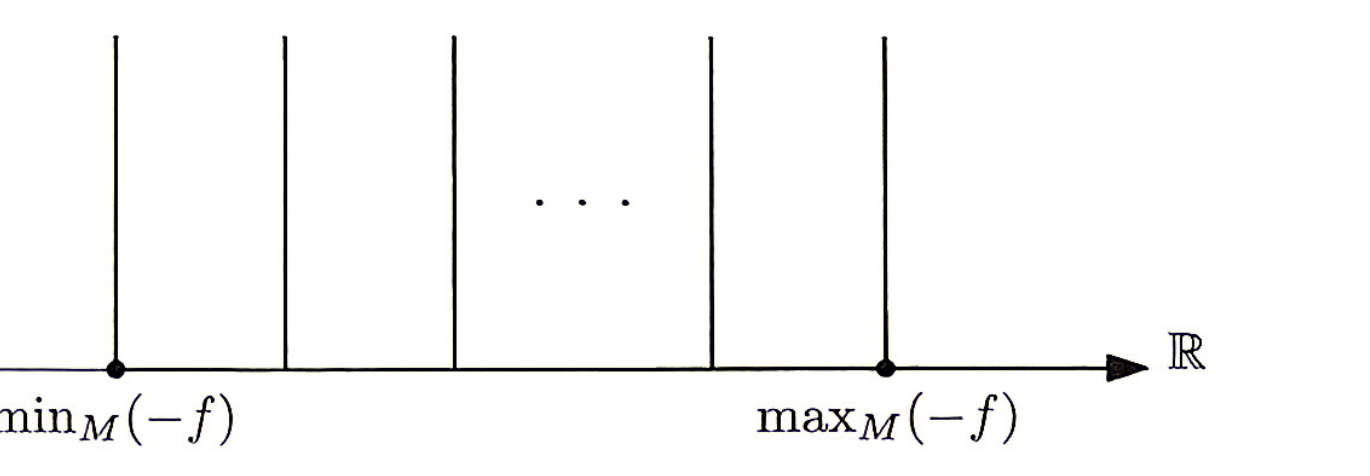
\includegraphics[width=0.66\linewidth]{figures/fig_p334_1.png}
  \caption*{图 10.10\quad (10.45) 的右端（原书 p.326, Figure 10.10；PDF p.334）}
\end{figure}

一个有趣的观察是：(10.45) 的右端作为 $SS(R\pi_*\mathcal F)$ 的上界，检测了
函数 $-f\colon M\to\R$ 的临界值。此外，由奇性支撑的定义，在每个临界值
$x\in M$（其中 $\mathrm df(x)=0$）处，层
$\mathcal F=\mathbf{k}_{\{(x,t)\mid f(x)+t\ge0\}}$ \emph{不}传播，其意义是
某些层上同调群会发生变化。回忆 5.2 节例 5.2.1：每当经过一个临界值，过滤
莫尔斯同调群 $\mathrm{HM}_*(\{f<t\};\mathbf{k})$ 就会改变。它如何改变，可以
有效地打包为在例 5.2.2 中定义的持续模 $\mathbb{V}_f$（并可由相应的条形码
图示）。在这个意义上，层（连同 $SS$）、持续模与莫尔斯理论彼此相关！
\hfill$\square$

\begin{wexer}{10.7.2}
  对零截面 $0_\R\subset T^*\R$（作为拉格朗日子流形），取 $0_\R$ 的、由
  \[
    S(x,e)=e^2
  \]
  定义的生成函数 $S\colon\R(x)\times\R(e)\to\R$。这里 $\R(x)$ 表示坐标 $x$
  下的一维欧氏空间 $\R$，$\R(e)$ 类似。考虑
  \[
    \mathcal F:=\mathbf{k}_{\{(x,e,t)\in\R(x)\times\R(e)\times\R(t)
    \mid S(x,e)\ge t\}},
  \]
  视作 $\Op{Ob}\bigl(D^+(\Op{Sh}(\mathbf{k}_{\R(x)\times\R(e)\times\R(t)}))
  \bigr)$ 中的一个（以 $0$ 次为中心的）复形，以及自然投影
  $p\colon\R(x)\times\R(e)\times\R(t)\to\R(x)\times\R(t)$。计算
  $Rp_!\mathcal F$ 与 $SS(Rp_!\mathcal F)$。论证经过一次约化后，
  $SS(Rp_!\mathcal F)$ 还原出拉格朗日子流形 $0_\R$。
\end{wexer}

下述结果汇集了奇性支撑在层上不同算子下的函子性态。

\begin{wprop}{10.7.3（[135] 中的命题 5.4.5 与命题 5.4.14）}
  (i) 若 $f\colon X\to Y$ 是淹没，则对
  $\mathcal F\in\Op{Ob}(D(\Op{Sh}(\mathbf{k}_Y)))$，
  \[
    SS(f^{-1}\mathcal F)=\bigl\{(x,p)\in T^*X\ \big|\
    \exists(y,\eta)\in SS(\mathcal F)\ \text{使得}\
    f(x)=y,\ f^*(\eta)=p\bigr\}.
  \]
  (ii) 对 $\mathcal F,\mathcal G\in\Op{Ob}(D(\Op{Sh}(\mathbf{k}_X)))$，若
  $SS(\mathcal F)\cap SS(\mathcal G)^a\subset0_X$（其中
  $SS(\mathcal G)^a$ 表示把 $SS(\mathcal G)$ 中余向量的符号取反），则
  \[
    SS(\mathcal F\otimes\mathcal G)\subset
    \bigl\{(x,\xi_1+\xi_2)\in T^*X\ \big|\
    (x,\xi_1)\in SS(\mathcal F),\ (x,\xi_2)\in SS(\mathcal G)\bigr\}.
  \]

% >>> p335
  (iii) 对 $\mathcal F,\mathcal G\in\Op{Ob}(D(\Op{Sh}(\mathbf{k}_X)))$，若
  $SS(\mathcal F)\cap SS(\mathcal G)\subset0_X$，则
  \[
    SS(R\Hom(\mathcal F,\mathcal G))\subset
    \bigl\{(x,-\xi_1+\xi_2)\in T^*X\ \big|\
    (x,\xi_1)\in SS(\mathcal F),\ (x,\xi_2)\in SS(\mathcal G)\bigr\}.
  \]
\end{wprop}

\begin{wexam}{10.7.3（参看例 10.7.1）}
  考虑由 $\delta(x)=(x,x)$ 定义的对角映射 $\delta\colon X\to X\times X$。则
  \[
    SS(\delta^{-1}\mathcal F)=\bigl\{(x,\eta_1+\eta_2)\in T^*X\ \big|\
    (x,\eta_1)\in T^*X,\ (x,\eta_2)\in T^*X\bigr\}.
  \]
  在某种程度上，例 10.7.1 中的求和 $s$ 表现得像是这里对角映射 $\delta$ 的
  「对偶」。\hfill$\square$
\end{wexam}

下述练习是命题 10.7.3 中 (i) 与 (ii) 的一个有用应用。

\begin{wexer}{10.7.3}
  给定 $X$ 与 $Y$，设
  $\mathcal F\in\Op{Ob}(D(\Op{Sh}(\mathbf{k}_X)))$，
  $\mathcal G\in\Op{Ob}(D(\Op{Sh}(\mathbf{k}_Y)))$，定义\textbf{外张量积}
  （external tensor product）为
  \[
    \mathcal F\boxtimes\mathcal G
    :=(p_1^{-1}\mathcal F)\otimes(p_2^{-1}\mathcal G),
  \]
  其中 $p_1\colon X\times Y\to X$、$p_2\colon X\times Y\to Y$ 是投影。
  然后验证
  \[
    SS(\mathcal F\boxtimes\mathcal G)\subset
    \bigl\{((x,p),(y,\eta))\in T^*X\times T^*Y\ \big|\
    (x,p)\in SS(\mathcal F)\ \text{且}\ (y,\eta)\in SS(\mathcal G)\bigr\},
  \]
  其中右端是 $SS(\mathcal F)$ 与 $SS(\mathcal G)$ 的笛卡尔积。
\end{wexer}

\begin{wrem}{10.7.2}
  在「奇性支撑把层转化为（奇）子流形」这一哲学下，练习 10.7.3 大致说明：
  几何中的笛卡尔积对应于层论中的外张量积。
\end{wrem}

% [Tutor Note: 术语依据——命题 10.7.3 汇集的是微局部层论中「六种运算」对
% 奇性支撑的作用：$f^{-1}$（拉回，淹没用等号）、$Rf_*$/$Rf_!$（前推，用固有性
% 与「存在投影」）、$\otimes$（张量积，需 $SS(\mathcal F)\cap SS(\mathcal G)^a
% \subset0_X$ 的横截性）、$R\mathcal H om$（内 Hom，需
% $SS(\mathcal F)\cap SS(\mathcal G)\subset0_X$）。注意 (ii) 中
% $SS(\mathcal G)^a$ 的上标 $a$ 专指「把余向量整体变号」，与取负集
% $-SS(\mathcal G)$ 记号不同，切勿混淆。]

下面我们引入层上的另一个运算，它综合了目前为止讨论的所有初等运算。

记 $p_i\colon X\times\R_1\times X\times\R_2\to X\times\R_i$ 为自然投影，
$i=1,2$。定义
\[
  s\colon X\times\R_1\times X\times\R_2\to X\times X\times\R,\qquad
  s\bigl((x,t_1),(y,t_2)\bigr)=(x,y,t_1+t_2).
\]
记对角映射 $\delta\colon X\times\R\to X\times X\times\R$，
$\delta(x,t)=(x,x,t)$。则对
$\mathcal F,\mathcal G\in\Op{Ob}(D(\Op{Sh}(\mathbf{k}_{X\times\R})))$，
如下定义\textbf{层卷积}（sheaf convolution）：
\begin{equation}\tag{10.46}
  \mathcal F*\mathcal G
  :=\delta^{-1}\bigl(Rs_!(\mathcal F\boxtimes\mathcal G)\bigr)
  =\delta^{-1}\bigl(Rs_!(p_1^{-1}\mathcal F\otimes p_2^{-1}\mathcal G)\bigr).
\end{equation}
几何上，层卷积运算由三步组成：$SS(\mathcal F)$ 与 $SS(\mathcal G)$ 的笛卡尔积
（由练习 10.7.3，对应于外张量积 $\boxtimes$）；在 $\R$ 中对具有相同余向量的
位置求和（由例 10.7.1，对应于固有前推 $Rs_!$）；在 $X$ 中对具有相同位置的
余向量求和（由例 10.7.3，对应于拉回 $\delta^{-1}$）。

让我们把层卷积应用到一个具体例子。

% >>> p336
\begin{wexam}{10.7.4}
  设 $f,g\colon X\to\R$ 是连续映射。由例 10.6.5，可以考虑
  \begin{equation}\tag{10.47}
    \mathcal F_f:=\mathbf{k}_{N_f}
    =\mathbf{k}_{\{(x,t)\mid f(x)+t\ge0\}}
    \in\Op{Ob}(D(\Op{Sh}(\mathbf{k}_{X\times\R}))),
  \end{equation}
  类似地有 $\mathcal F_g$。回忆
  $SS(\mathcal F_f)=0_{N_f}\cup
  \{(x,\tau\mathrm df(x),-f(x),\tau)\mid x\in X,\tau>0\}$ 以及
  $SS(\mathcal F_g)=0_{N_g}\cup
  \{(x,\tau\mathrm dg(x),-g(x),\tau)\mid x\in X,\tau>0\}$。为计算
  $SS(\mathcal F_f*\mathcal F_g)$，我们将逐步进行这一过程。首先，
  \[
    SS(\mathcal F_f\boxtimes\mathcal F_g)\subset
    \bigl\{\bigl((x,\tau_1\mathrm df(x),-f(x),\tau_1),
    (y,\tau_2\mathrm dg(y),-g(y),\tau_2)\bigr)\ \big|\
    x,y\in X,\ \tau_1,\tau_2>0\bigr\}.
  \]
  第二，由 $Rs_!$ 得到
  \[
    SS\bigl(Rs_!(\mathcal F_f\boxtimes\mathcal F_g)\bigr)\subset
    \bigl\{(x,\tau\mathrm df(x),y,\tau\mathrm dg(y),-f(x)-g(y),\tau)\ \big|\
    x,y\in X,\ \tau>0\bigr\}.
  \]
  第三，由 $\delta^{-1}$ 得到
  \begin{align*}
    SS(\mathcal F_f*\mathcal F_g)
    &\subset\bigl\{(x,\tau\mathrm d(f+g)(x),-f(x)-g(x),\tau)\ \big|\
      x\in X,\ \tau>0\bigr\}\\
    &=SS(\mathcal F_{f+g}).
  \end{align*}
  这意味着在这一设定下，层卷积在几何上对应于逐纤维求和。\hfill$\square$
\end{wexam}

\begin{wexer}{10.7.4}
  对 (10.46) 中定义在 $D(\Op{Sh}(\mathbf{k}_{X\times\R}))$ 上的层卷积，设
  $X=\{\mathrm{pt}\}$，计算 $\mathbf{k}_{[a,b]}*\mathbf{k}_{[c,d]}$（区间
  $[a,b],[c,d]\subset\R$）。可随意使用如下事实：对任何
  $\mathcal F\in\Op{Ob}(\Op{Sh}(\mathbf{k}_X))$，有
  $\mathcal F\otimes\mathbf{k}_Z\simeq\mathcal F_Z$（任何局部闭子集
  $Z\subset X$）。
\end{wexer}

下面，我们再引入另一个运算。考虑流形之积 $X_1\times X_2\times X_3$ 与自然
投影 $\pi_{ij}\colon X_1\times X_2\times X_3\to X_i\times X_j$，其中
$(i,j)=(1,2),(1,3)$ 或 $(2,3)$。则对
$\mathcal F\in\Op{Ob}(D(\Op{Sh}(\mathbf{k}_{X_1\times X_2})))$、
$\mathcal G\in\Op{Ob}(D(\Op{Sh}(\mathbf{k}_{X_2\times X_3})))$，如下定义
$\mathcal F$ 与 $\mathcal G$ 的\textbf{层复合}（sheaf composition）
\begin{equation}\tag{10.48}
  \mathcal F\circ\mathcal G
  :=R\pi_{13!}\bigl(\pi_{12}^{-1}\mathcal F
  \otimes\pi_{23}^{-1}\mathcal G\bigr)
  \in\Op{Ob}(D(\Op{Sh}(\mathbf{k}_{X_1\times X_3}))).
\end{equation}
与层卷积 (10.46) 类似，我们可以逐步研究层复合「$\circ$」的几何意义。首先，
由命题 10.7.3 中的 (i)，
\[
  SS(\pi_{12}^{-1}\mathcal F)=\left\{(x_1,x_2,x_3,p_1,p_2,p_3)\ \middle|\
  \begin{array}{l}
    \exists(y_1,y_2,\eta_1,\eta_2)\in SS(\mathcal F)\ \text{s.t.}\\
    \pi_{12}(x_1,x_2,x_3)=(y_1,y_2),\\
    \pi_{12}^*(\eta_1,\eta_2)=(p_1,p_2,p_3)
  \end{array}\right\}
\]
\[
  =\bigl\{(y_1,y_2,x_3,\eta_1,\eta_2,0)\ \big|\
  (y_1,y_2,\eta_1,\eta_2)\in SS(\mathcal F),\ x_3\in X_3\bigr\}.
\]
类似地，
\[
  SS(\pi_{23}^{-1}\mathcal G)
  =\bigl\{(x_1,y_2,y,0,\eta_2,\eta_3)\ \big|\
  (y_2,y_3,\eta_2,\eta_3)\in SS(\mathcal G),\ x_1\in X_1\bigr\}.
\]

% [Tutor Note: 原文疑误——上式元组 $(x_1,y_2,y,0,\eta_2,\eta_3)$ 中的第三个
% 分量原文印作 $y$，但按前一行「$(y_2,y_3,\eta_2,\eta_3)\in SS(\mathcal G)$」
% 与 $\pi_{23}\colon X_1\times X_2\times X_3\to X_2\times X_3$ 的坐标安排，
% 该分量应为 $y_3$。此处保留原文写法并已记入审校记录。]

% >>> p337
第二，由于 $SS(\pi_{12}^{-1}\mathcal F)\cap SS(\pi_{23}^{-1}\mathcal G)^a
=0_{X_1\times X_2\times X_3}$，由命题 10.7.3 我们有
\[
  SS(\pi_{12}^{-1}\mathcal F\otimes\pi_{23}^{-1}\mathcal G)\subset
  \left\{(y_1,y_2,y_3,\eta_1,\eta_2+\eta_2',\eta_3)\ \middle|\
  \begin{array}{l}
    (y_1,y_2,\eta_1,\eta_2)\in SS(\mathcal F)\\
    (y_2,y_3,\eta_2',\eta_3)\in SS(\mathcal G)
  \end{array}\right\}.
\]
第三，由命题 10.7.2 我们有
\[
  SS(\mathcal F\circ\mathcal G)\subset\left\{
  (x_1,x_3,p_1,p_3)\ \middle|\
  \begin{array}{l}
    \exists(y_1,y_2,y_3,\eta_1,\eta_2,\eta_3)
    \in SS(\pi_{12}^{-1}\mathcal F\otimes\pi_{23}^{-1}\mathcal G)\\
    \text{使得}\ \pi_{13}(y_1,y_2,y_3)=(x_1,x_3)\\
    \text{且}\ \pi_{13}^*(p_1,p_3)=(\eta_1,\eta_2,\eta_3)
  \end{array}\right\}
\]
\[
  =\left\{(y_1,y_3,\eta_1,\eta_3)\ \middle|\
  \begin{array}{l}
    \exists(y_1,y_2,\eta_1,\eta_2)\in SS(\mathcal F)\\
    (y_2,y_3,-\eta_2,\eta_3)\in SS(\mathcal G)
  \end{array}\right\}.
\]
事实上，最后一步是一个众所周知的几何运算：给定任意两个闭（锥）子集
$\Lambda_1\subset T^*(X_1\times X_2)$、$\Lambda_2\subset T^*(X_2\times X_3)$，
如下定义它们的\textbf{拉格朗日对应}（Lagrangian correspondence）
\begin{equation}\tag{10.49}
  \Lambda_1\circ\Lambda_2:=\left\{
  (y_1,y_3,\eta_1,\eta_3)\in T^*(X_1\times X_3)\ \middle|\
  \begin{array}{l}
    \exists(y_2,\eta_2)\in T^*X_2\ \text{使得}\\
    (y_1,y_2,\eta_1,\eta_2)\in T^*(X_1\times X_2)\\
    (y_2,y_3,-\eta_2,\eta_3)\in T^*(X_2\times X_3)
  \end{array}\right\}.
\end{equation}
于是我们得到的是
\begin{equation}\tag{10.50}
  SS(\mathcal F\circ\mathcal G)\subset SS(\mathcal F)\circ SS(\mathcal G),
\end{equation}
这意味着层复合对应于拉格朗日对应。

下述例子表明，层复合可用来在（导出）层范畴上表述一个运算。

\begin{wexam}{10.7.5}
  在层复合 (10.48) 的设定中，设 $X_3=\{\mathrm{pt}\}$，$X_1=X_2=X$。
  对一个固定对象 $\mathcal F\in\Op{Ob}(D(\Op{Sh}(\mathbf{k}_{X\times X})))$，
  考虑任何 $\mathcal G\in\Op{Ob}(D(\Op{Sh}(\mathbf{k}_{X\times\{\mathrm{pt}\}})))
  =\Op{Ob}(D(\Op{Sh}(\mathbf{k}_X)))$，我们有
  \[
    \mathcal F\circ\mathcal G\in\Op{Ob}(D(\Op{Sh}(\mathbf{k}_X))).
  \]
  换言之，$\mathcal F\circ$ 充当作用在 $D(\Op{Sh}(\mathbf{k}_X))$ 上的一个
  运算。\hfill$\square$
\end{wexam}

下面这个例子承接例 10.7.5，演示如何把哈密顿同痕的作用转化为层语言。

\begin{wexam}{10.7.6}
  给定齐次哈密顿同痕 $\Phi=\{\varphi_H^t\}\colon I\times\dot T^*X
  \to\dot T^*X$，取定理 10.6.1 中的 GKS 层量子化
  $\mathcal K_\Phi\in\Op{Ob}(D(\Op{Sh}(\mathbf{k}_{X\times X\times I})))$
  （以及它在 $t_*\in I$ 处的限制
  $\mathcal K_\Phi|_{t=t_*}\in\Op{Ob}(D(\Op{Sh}(\mathbf{k}_{X\times X})))$）。
  对 $\mathcal F\in\Op{Ob}(D(\Op{Sh}(\mathbf{k}_X)))$，仿照例 10.7.5，我们将
  考虑
  \[
    \mathcal K_\Phi|_{t=t_*}\circ\mathcal F
    \in\Op{Ob}(D(\Op{Sh}(\mathbf{k}_X))).
  \]
\end{wexam}

% >>> p338
由 (10.50) 与定理 10.6.1 中的 (i)，我们有
\[
  SS(\mathcal K_\Phi|_{t=t_*}\circ\mathcal F)
  \subset SS(\mathcal K_\Phi|_{t=t_*})\circ SS(\mathcal F)
  \subset\bigl(\Lambda_\Phi|_{t=t_*}\cup0_{X\times X}\bigr)\circ SS(\mathcal F),
\]
其中
$\Lambda_\Phi|_{t=t_*}=\bigl\{((x,p),-\varphi_H^{t_*}(x,p))\ \big|\
(x,p)\in\dot T^*X\bigr\}$。此外，由 (10.49)，
\[
  \Lambda_\Phi|_{t=t_*}\circ SS(\mathcal F)
  =\left\{(x,p)\in T^*X\ \middle|\
  \begin{array}{l}
    \exists(y,\eta)\in SS(\mathcal F)\cap\dot T^*X\ \text{使得}\\
    ((x,p),(y,\eta))\in\Lambda_\Phi|_{t=t_*}
  \end{array}\right\}
  =\varphi_H^{-t_*}\bigl(SS(\mathcal F)\cap\dot T^*X\bigr).
\]
此外，
\[
  0_{X\times X}\circ SS(\mathcal F)
  =\left\{(x,p)\in T^*X\ \middle|\
  \begin{array}{l}
    \exists(y,\eta)\in SS(\mathcal F)\ \text{使得}\\
    ((x,p),(y,\eta))\in0_{X\times X}
  \end{array}\right\}=0_X.
\]
因此我们断言
\begin{equation}\tag{10.51}
  SS(\mathcal K_\Phi|_{t=t_*}\circ\mathcal F)
  \subset\varphi_H^{-t_*}\bigl(SS(\mathcal F)\cap\dot T^*X\bigr)\cup0_X.
\end{equation}
几何上，GKS 层量子化「$\mathcal K_\Phi|_{t=t_*}\circ$」的作用对应于哈密顿
微分同胚 $\varphi_H^{-t_*}$ 的作用。\hfill$\square$
